\scanpage{53}
% archive sheet number: 52

% printed form
\texttt{//*\quad CRAY2\quad 0411\qquad I}

{\scriptsize
\begin{verbatim}
           00000000      00000000      00000000      00000000
         0000000000    0000000000    0000000000    0000000000
       00      0000  00      0000  00      0000  00      0000
      00     00 00  00     00 00  00     00 00  00     00 00
     00    00  00  00    00  00  00    00  00  00    00  00
    00   00   00  00   00   00  00   00   00  00   00   00
   00  00    00  00  00    00  00  00    00  00  00    00
  00 00     00  00 00     00  00 00     00  00 00     00
 0000      00  0000      00  0000      00  0000      00
000       00  000       00  000       00  000       00
0000000000    0000000000    0000000000    0000000000
00000000      00000000      00000000      00000000
\end{verbatim}
}

{\scriptsize
\begin{verbatim}
 CCCCCCCCCC   RRRRRRRRRRR    AAAAAAAAAA   YY        YY   2222222222
CCCCCCCCCCCC  RRRRRRRRRRRR  AAAAAAAAAAAA  YY        YY  222222222222
CC        CC  RR        RR  AA        AA   YY      YY   22        22
CC            RR        RR  AA        AA    YY    YY              22
CC            RR        RR  AA        AA     YY  YY               22
CC            RRRRRRRRRRRR  AAAAAAAAAAAA      YYYY               22
CC            RRRRRRRRRRR   AAAAAAAAAAAA       YY              22
CC            RR    RR      AA        AA       YY            22
CC            RR     RR     AA        AA       YY          22
CC        CC  RR      RR    AA        AA       YY        22
CCCCCCCCCCCC  RR       RR   AA        AA       YY       222222222222
 CCCCCCCCCC   RR        RR  AA        AA       YY       222222222222
\end{verbatim}
}

{\fontsize{4.5}{5.9}\selectfont
\begin{verbatim}
****A  START  JOB  411  CRAY2                           ROOM        4.18.41 PM 16 AUG 82  R6.PR1    SYS JES2  JOB  411  START  A****
****A  START  JOB  411  CRAY2                           ROOM        4.18.41 PM 16 AUG 82  R6.PR1    SYS JES2  JOB  411  START  A****
****A  START  JOB  411  CRAY2                           ROOM        4.18.41 PM 16 AUG 82  R6.PR1    SYS JES2  JOB  411  START  A****
****A  START  JOB  411  CRAY2                           ROOM        4.18.41 PM 16 AUG 82  R6.PR1    SYS JES2  JOB  411  START  A****
****A  START  JOB  411  CRAY2                           ROOM        4.18.41 PM 16 AUG 82  R6.PR1    SYS JES2  JOB  411  START  A****
****A  START  JOB  411  CRAY2                           ROOM        4.18.41 PM 16 AUG 82  R6.PR1    SYS JES2  JOB  411  START  A****
\end{verbatim}
}

\texttt{DERNIERE MISE A JOUR DE JOURNAL : 11-08-82}\\
\texttt{ATTENTION ...........}

\texttt{1. ARRET DE L'ORDINATEUR LE MARDI 17 AOUT DE 7 H A 8 H.}

\texttt{] \quad 2. UNE MODIFICATION SYSTEME NOUS CONTRAINDRA A DETRUIRE}\\
\texttt{] \qquad LE CONTENU DU DISQUE SPOOL LE MARDI 17 AOUT A 6 HEURES}\\
\texttt{] \qquad VEUILLEZ RECUPERER VOS SORTIES EN ATTENTE AVANT CETTE}\\
\texttt{] \qquad DATE. MERCI DE VOTRE COMPREHENSION.}

\texttt{] \quad 3. UN ARRET EXCEPTIONNEL POUR PREPARER L'ARRIVEE DE NOUVELLES}\\
\texttt{] \qquad UNITES AURA LIEU DU VENDREDI 20 AOUT A 17H 3\unsure{0} AU LUNDI}\\
\texttt{] \qquad 23 AOUT A 8H.}

\figure{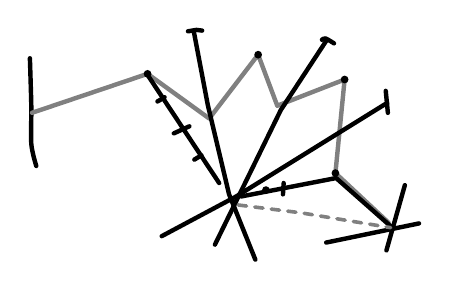
\begin{tikzpicture}[x=0.009cm,y=-0.009cm,line cap=round,line join=round]
\draw[line width=1.6pt] plot[smooth] coordinates {(6,45) (8,113) (8,166) (15,197)};
\draw[gray,line width=1.6pt] (9,122)--(172,67)--(259,130)--(328,40)--(355,112)--(450,75)--(437,207)--(512,277);
\draw[line width=1.6pt] (171,67)--(273,221);
\draw[line width=1.6pt] (186,106)--(196,100);
\draw[line width=1.6pt] (209,151)--(231,141);
\draw[line width=1.6pt] (238,188)--(248,182);
\draw[line width=1.6pt] (229,7)--(241,5)--(249,6);
\draw[line width=1.6pt] (237,6)--(257,111)--(287,237)--(324,329);
\draw[line width=1.6pt] plot[smooth] coordinates {(418,19) (423,17) (435,24)};
\draw[line width=1.6pt] (425,19)--(360,118)--(267,308);
\draw[line width=1.6pt] (192,296)--(297,240)--(510,108);
\draw[line width=1.6pt] (508,91)--(511,122);
\draw[line width=1.6pt] (304,240)--(438,214)--(515,282);
\draw[line width=1.6pt] (535,224)--(509,316);
\draw[line width=1.6pt] (424,305)--(555,278);
\draw[gray,line width=1.3pt,dashed] (300,252)--(388,263)--(515,284);
\draw[line width=1.6pt] (364,221)--(363,237);
\fill[black] (172,67) circle [radius=1.4pt];
\fill[black] (328,40) circle [radius=1.4pt];
\fill[black] (450,75) circle [radius=1.4pt];
\fill[black] (437,207) circle [radius=1.4pt];
\fill[black] (339,231) circle [radius=1.4pt];
\end{tikzpicture}}

\figure{\begin{tikzpicture}[x=0.006cm,y=-0.006cm,line cap=round,line join=round]
\draw[thin] plot[smooth] coordinates {(170,0) (105,127) (48,272) (10,430) (5,598) (29,744)};
\end{tikzpicture}}

\figure{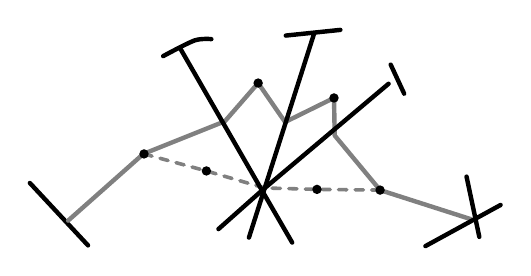
\begin{tikzpicture}[x=0.009cm,y=-0.009cm,line cap=round,line join=round]
\draw[line width=1.6pt] (0,224)--(82,312);
\draw[gray,line width=1.6pt] (54,277)--(160,183)--(275,137)--(322,83)--(360,138)--(429,104)--(430,157)--(494,234)--(622,275);
\draw[gray,line width=1.3pt,dashed] (161,183)--(249,207)--(331,231)--(405,233)--(494,234);
\draw[line width=1.6pt] plot[smooth] coordinates {(188,45) (232,23) (256,21)};
\draw[line width=1.6pt] (212,34)--(326,232)--(370,308);
\draw[line width=1.6pt] (361,16)--(438,8);
\draw[line width=1.6pt] (401,13)--(309,301);
\draw[line width=1.6pt] (266,289)--(328,234)--(506,84);
\draw[line width=1.6pt] (509,57)--(528,98);
\draw[line width=1.6pt] (558,313)--(664,255);
\draw[line width=1.6pt] (616,215)--(634,300);
\fill[black] (161,183) circle [radius=1.7pt];
\fill[black] (249,207) circle [radius=1.7pt];
\fill[black] (322,83) circle [radius=1.7pt];
\fill[black] (429,104) circle [radius=1.7pt];
\fill[black] (405,233) circle [radius=1.7pt];
\fill[black] (494,234) circle [radius=1.7pt];
\end{tikzpicture}}
